\chapter{A multi-view modeling framework\label{chapter:framework}}

This chapter installs the background necessary for understanding subsequent chapters of this thesis. 

\newcommand{\artifact}[1]{\texttt{#1}}

\section{Running example: A toy train system}

We use a simple train system fragment as running example for illustrating concepts and techniques throughout this thesis. The system is composed of an automated train controller, actuators for doors and the engine as well as the latter themselves, sensors, and a passenger. Via the actuators, the controller typically controls operations like starting or stopping the train, opening or closing the doors, and so on. A safety goal requires train doors to remain closed while the train is moving. If the train is not moving and the passenger presses the alarm button, the controller must open the doors immediately. If the train is moving and the passenger presses the alarm button, then the controller must stop the train first and then open the doors. Typical agent interactions for the latter case are depicted in Fig.~\ref{image:train-scenario-all-agents}. The precise semantics of such a scenario is made clear in the following sections.

\begin{figure}[H]\centering
\scalebox{0.75}{
  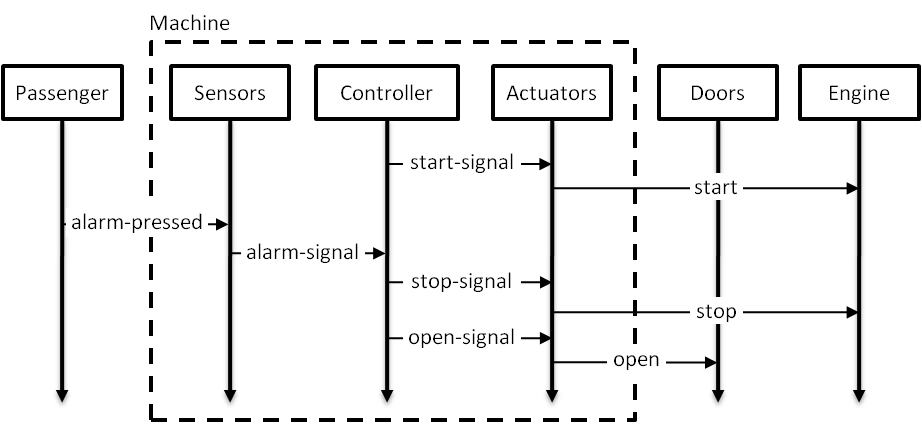
\includegraphics{src/2-framework/images/train-scenario-all-agents}
}
\caption{A scenario illustrating a train system stopping in emergency when an alarm is pressed.\label{image:train-scenario-all-agents}}
\end{figure}

\section{Agents, System and their Behavior}

A system is commonly admitted to be made of active components, called \emph{agents}, that behave and interact so as to fulfill system goals while restricting their behavior to ensure constraints they are assigned to~\cite{Feather:1987}. Some of them are human agents (the passenger), others are physical or electronic devices (e.g. the doors, the actuators), still others are software components (the automated controller). In addition to the notion of \emph{system}, that encompass all agents, the literature makes use of specific terms to distinguish between certain agents and/or agent aggregations. In~\cite{VanLamsweerde:2009} for example, the \emph{software-to-be} denotes software agent(s) that need to be developed (the automated controller, for example), while other agents compose its \emph{environment}. Another boundary consists in distinguishing the software together with its input and output devices from other agents. This boundary, depicted with a dashed line in Fig.~\ref{image:train-scenario-all-agents}, corresponds to the distinction made by Jackson between the \emph{world} and the \emph{machine}~\cite{Jackson:1995}. In this thesis, we focus on the behavior of a single agent as observed by the other agents with which it interacts (as opposed to its internal implementation). From the former agent perspective, then, the \emph{environment} is made of all these latter agents. 

In the light of the previous paragraph, we clearly need tools to capture single agent behaviors while being able to play with agent boundaries in a flexible manner -- for instance, for ``computing'' the behavior of agent aggregations like the \emph{software environment}, the \emph{machine} or simply, the \emph{system}. For this, we choose to model behaviors and interactions in an event-based framework, where agents communicate via messages that are sent and received simultaneously. Such kind of communication, called \emph{synchronous communication} or simply, \emph{message passing}, is motivated by its simplicity, an important aspect for accessibility to stakeholders involved during the early-design phase of a system. The next section introduces  labeled transition systems (LTS), the kind of model we use to capture agent behaviors. The next one presents operators for composing (and decomposing) them under a \emph{synchronous communication} hypothesis, a manner of capturing the behaviors of multiple interacting agents.

\subsection{Agents as Labeled Transition Systems}

In our framework, the behavior of an agent, say \artifact{Ag}, is modeled by a specific kind of finite state machine, called \emph{labeled transition system} (LTS). This formalism, initially introduced by Keller for reasoning about parallel programs~\cite{Keller:1976}, has since been intensively used for specifying and analyzing concurrent systems, e.g. in~\cite{Milner:1989, Clarke:1989, Magee:1997}. A LTS is made of a set of states and a set of transitions between them (see Fig.~\ref{image:framework-start-stop}). Each transition is depicted with an \emph{event} label -- sometimes called an \emph{action} label; also, a specific state is the \emph{initial state}, designated graphically by an empty arrow in front of it (state 0 in the figure). 

\vspace{0.5cm}
\begin{figure}[H]
\centering\scalebox{0.60}{
  \includegraphics*[clip]{src/2-framework/images/start-stop}}
  \caption{A Labeled Transition System for an \artifact{Engine} agent\label{image:framework-start-stop}.}
\end{figure}

Labeled transition systems come with different flavors in the literature that allows capturing more or less meaning, also resulting in few or numerous semantics subtleties. We stick here with a very simple framework, by restricting our attention to \emph{determinate} agents~\cite{Engelfriet:1985}, that is, agents whose behavior can be modeled using \emph{deterministic} transition systems (see below). While a somewhat restrictive choice in terms of expressiveness --~many approaches arising from process algebra do not restrict to such an hypothesis~-- we argue that it naturally keeps the framework simple and intuitive to use for stakeholders. We now turn to some mathematical definitions that, among others, define the aforementioned terms.

Mathematically, a LTS is defined as a 4-tuple $(Q,\Sigma,\delta,q_{init})$ where $Q$ is a finite set of states, $\Sigma$ is a set of labels called its \emph{alphabet}, $\delta$ is a transition relation $Q \times \Sigma\cup\{\tau\} \times Q$ and $q_{init} \in Q$ is the initial state.

A \emph{deterministic} LTS does not have $\tau$ transitions and has no state with two outgoing transitions having the same label (that is, $(q,l,q_1) \in \delta \wedge (q,l,q_2) \in \delta \implies q_1 = q_2$); otherwise it is \emph{non-deterministic}.

A \emph{terminating} LTS has at least one state with no outgoing transition, otherwise it is \emph{non-terminating}. This notion naturally extends to terminating and non-terminating \emph{states}. Note that, as such, the LTS definition does not allow distinguishing between terminating states that model successful termination -- an agent stops running intentionally -- and non-successful termination -- an agent, more often the system as a \emph{composed} agent (see next section), \emph{deadlocks} unintentionally. We will come back to this discussion in section~\ref{section:background-discussion}.

The \emph{alphabet} $\Sigma$ captures the notion of \emph{agent interface}, as a set of event labels that an agent recognizes or, said otherwise, in which the agent \emph{engages} in synchronous communications with its environment. For example, the LTS of Fig.~\ref{image:framework-start-stop} has an alphabet \artifact{$\Sigma=\{start, stop\}$}. Note that labeled transition systems do not distinguish between \emph{sent} and \emph{received} events. This distinction being required when playing with scenarios, we assume that an event label uniquely determines the interacting agents and that this architectural information is available elsewhere (typically, from the scenarios themselves). However, we allow an event label to be shared between more than two agents, but assume that only one of them is the \emph{sender}. By simplicity in the sequel, we denote $\Sigma\cup\{\tau\}$ by $\Sigma_{\tau}$ (an alphabet augmented with the $\tau$ label).

An finite LTS \emph{execution} is a finite sequence of its states separated by labels, i.e. \artifact{$w = \textless q_0,l_0,\ldots,q_{n-1},l_{n-1},q_n \textgreater$} with $q_i \in Q$ and $l_i \in \Sigma_{\tau}$. An execution is valid for a LTS if it denotes an existing path, from the initial state, in the corresponding graph; mathematically, $q_0 = q_{init}$ and $(q_i,l_i,q_{i+1}) \in \delta$ for $0 \leq i < n$. The projection of an execution $w$ over an alphabet $\Sigma$ is denoted by $w|_{\Sigma}$ and is the result of keeping, from $w$, only event labels that belong to $\Sigma$ (in other words, eliminating $q_i$ states and $\tau$ labels). Such a projection is also called a \emph{trace}, that we define now.

A \emph{trace} denotes an element of $\Sigma^*$, that is a finite sequence of event labels \artifact{$t= \textless l_0,\ldots,l_{n} \textgreater$} with $l_i \in \Sigma$. Unlike an execution, a trace never contains $\tau$ labels. A trace $t$ is accepted by a LTS if there exists a valid execution $w$ such that $w|_{\Sigma} = t$. In other words, a trace is \emph{accepted} by a LTS if it denotes an existing path in the corresponding graph from the initial path, but allowing ``in the middle'' silent moves offered by $\tau$ transitions in the non-deterministic case (and hence, possibly, more than one path). Note that, by this definition, a prefix of an accepted trace is also an accepted trace; the empty trace $\lambda$ is therefore always accepted. For example, the LTS of Fig.~\ref{image:framework-start-stop} accepts the trace \artifact{<start stop start>}, and hence \artifact{<start stop>}, but not \artifact{<start start>}

The set of traces accepted by a LTS, say $P$, is called its \emph{language} and will be noted $\mathcal{L}(P)$. We naturally extend this notion to the language of an agent. For example, the  \emph{language} of the \artifact{Engine} agent is $\mathcal{L}(\artifact{Engine})=\{\lambda$, \artifact{<start>}, \artifact{<start stop>}, \artifact{<start stop start>}, \ldots $\}$. Actually, as prefixes of accepted traces are also accepted traces, LTS capture the class of \emph{prefix-closed} languages, a subclass of \emph{regular} languages~\cite{Hopcroft:1979}. This result opens the way of applying regular learning for synthesizing LTS, as detailed in chapter~\ref{chapter:inductive-synthesis}.

However, another important notion is the one of LTS \emph{equivalence} that permits answering questions like ``\emph{are agents $Ag_1$ and $Ag_2$ the same in term of their behavior?}''. Many different notions of behavioral equivalence exist in the literature, like \emph{strong} and \emph{observational}  equivalences~\cite{Milner:1989}. Their introduction (in process algebra) is motivated by the need to distinguish between particular process cases as well as being able reason about their correctness (in terms of \emph{deadlock}, for instance), especially when dealing with non-determinism. For details, see e.g.~\cite[chap. 3]{Hoare:1985}, \cite[chap. 4 \& 5]{Milner:1989} or the overview given in~\cite{Fernandez:1991}. Our hypotheses, especially the one of \emph{determinate} agents, allows us to stick with the weakest, yet simplest, notion of LTS equivalence: \emph{trace equivalence}~\cite{Hoare:1985, Engelfriet:1985}. Under the latter, two LTS $P$ and $Q$ are equivalent, denoted by $P \equiv_{tr} Q$, if they accept the same set of traces, in other words, if they define the same language $\mathcal{L}(P) = \mathcal{L}(Q)$. This definition naturally extends to behaviorally equivalent \emph{agents}.

Interestingly enough, under trace equivalence, many results from standard automata theory safely apply to LTS (that is, on can use them while preserving behavior equivalence). We revisit those classical results and other definitions in terms of agents and their behaviors. Section~\ref{section:inductive-background} later summarizes results specific to regular induction, where we need them. 

First, if we consider \emph{determinate} agents exclusively, it does not necessarily mean that we use only \emph{deterministic} LTS. Recall that, by definition, non-determinism naturally arises as soon as one uses $\tau$ transitions, and we sometimes do (see, in particular, the \emph{hiding} operator of next section). This apparent contradiction resolves naturally in our context. Indeed, given a non-deterministic LTS, it is always possible to find a deterministic one --hence, without any $\tau$ -- which is trace equivalent~\cite{Hopcroft:1979}.

Also, the notion of equivalence between two LTS can be revisited in terms of the states of a single LTS. For this, consider a LTS $P = (Q,\Sigma,\delta,q_{init})$ and an existing transition from its initial state $(q_{init},l,q_2) \in \delta$ with $l \in \Sigma_{\tau}$. It is often convenient to interpret this as the LTS $P$ that \emph{transits} with the label $l$ into the LTS $P' = (Q,\Sigma,\delta,q_{2})$. We denote this by $P \stackrel{l}{\longrightarrow} P'$ (which is also straightforward to generalize to accepted traces $P \stackrel{\textless s \textgreater}{\longrightarrow} P''$).  Observe that $P'$ is in fact the same transition system than $P$, except for the initial state. Now, it might be the case that $P$ and $P'$ are trace equivalent, and more generally, that a trace exists such that $P \equiv_{tr} P''$. If they are, it means that at least two states of the original LTS are trace equivalent, that is, that they ``generate'' the same language. From standard automaton theory, it is however possible to find a deterministic LTS accepting exactly the same set of traces but for which no such two states exist. Moreover, this LTS is minimal in terms of number of states and is unique up to state renumbering~\cite{Gold:1978}.

To sum up, any LTS $P$ -- being deterministic or not -- has a canonical deterministic and minimal form, up to state renumbering, that preserves behaviors. We denote it by $P^{\Delta}$. Unless stated otherwise, we consider that agent behaviors are captured by such an LTS, and use standard automaton algorithms in~\cite{Hopcroft:1979} -- when needed -- to remove $\tau$ transitions, determinize and minimize LTS. This also applies to LTS capturing behaviors of composed agents, that we introduce in next section. 

\subsection{System as Agent composition}

If a system is composed of active agents and the behavior of each of these agents is explicitly modeled with an LTS, one can ask what is the behavior of the system itself. We define it through parallel composition~\cite{Hoare:1985}, a setting where agents execute asynchronously but synchronize on shared events. Given a system made of $n$ agents, and the composition operator denoted by~$\parallel$, the system is defined as:

\begin{equation}
System = Ag_1 \parallel \ldots \parallel Ag_n
\end{equation}

As we are mostly interrested in agent \emph{behaviors}, we use the binary composition operator $\parallel$ defined on LTS, see e.g.~\cite{Giannakopoulou:1999, Magee:1999}. The operator, which is both commutative and associative (allowing our writing above without ambiguity), computes the interleaving of the traces accepted by the two LTS, under the constraint that they synchronize on shared labels. Let $P = (S_1,\Sigma_1,\delta_1,q_{1})$ and $Q = (S_2,\Sigma_2,\delta_2,q_{2})$ denote two LTS. Then, their composition $P \parallel Q$ is another LTS $(S_1 \times S_2,\Sigma_1\cup\Sigma_2,\delta,(q_1,q_2))$, where $\delta$ is the smallest relation satisfying the following rules:

\begin{center}
\begin{tabular}{cc}
$\frac{\displaystyle P \stackrel{l}{\longrightarrow} P'}{\displaystyle P \parallel Q \stackrel{l}{\longrightarrow} P' \parallel Q}~~l \notin \Sigma_2$ &
$\frac{\displaystyle Q \stackrel{l}{\longrightarrow} Q'}{\displaystyle P \parallel Q \stackrel{l}{\longrightarrow} P \parallel Q'}~~l \notin \Sigma_1$ \\
 & \\
\multicolumn{2}{c}{$\frac{\displaystyle P \stackrel{l}{\longrightarrow} P',~Q \stackrel{l}{\longrightarrow} Q'}{\displaystyle P \parallel Q \stackrel{l}{\longrightarrow} P' \parallel Q'}~~l \neq \tau$} \\
\end{tabular}
\end{center}

As one can see, $P \parallel Q$ is defined on the cartesian product of the states of $P$ and $Q$, and has its initial state simply defined as $(q_1,q_2)$ in this state space. Rules above define the possible transitions in such a state. The first two rules are symetric and encode the fact that, on non shared labels, one LTS transits while the other stay in its previous state. As stated, those rules allow individual LTS to move along $\tau$ transitions. The last rule forces the two LTS to transit together on all shared labels but $\tau$. A composed LTS can easily be computed constructively by exploring the state space from its initial state until no new state pair is discovered. The trace semantics of a system composed of $n$ agents whose behavior is modeled with LTSs $Ag_1$ to $Ag_n$ is captured as:

\begin{equation}
\mathcal{L}(System) = \mathcal{L}(Ag_1 \parallel \ldots \parallel Ag_n)
\label{equation:system-composition}
\end{equation}

\subsection{Black-box behavior through \emph{hiding}}

If the notion of agent composition gives a sound interpretation to the notion of \emph{system} and its behavior, it is, in fact, of slighlty more general use. Indeed, as explained in the introduction of this section, it makes sense to consider not only the composition of all agents but sometimes the composition of a subset of them that, together, define an interesting boundary in the system considered. Consider the agents depicted in the scenario of Fig.~\ref{image:train-scenario-all-agents} for example, and assume that $Controller$, $Actuators$, etc. actually denote their respective LTS. The ``machine vs. world'' boundary can simply be modeled as follows:

\vspace{-0.8cm}
\begin{align*}
Machine &= Controller \parallel Actuators \parallel Sensors \\
World   &= Passenger \parallel Doors \parallel Engine \\
System  &= Machine \parallel World
\end{align*}
\vspace{-0.8cm}

However, as defined above, the $Machine$ agent has an interface -- in terms of the set of events in which it engages -- which is actually too large. A look at the boundary depicted by the dashed line in Fig.~\ref{image:train-scenario-all-agents} clearly shows that some of its events model internal communications -- that is events between agents composing the Machine, like \artifact{start-signal} or \artifact{alarm-signal}) -- while other events form the natural interface of the $Machine$ with its environment -- those ``crossing'' the depicted boundary, like \artifact{alarm-pressed} or \artifact{stop}. It is often convenient to enforce this separation between internal and external interfaces, for example to avoid environment agents to synchronize with internal events. In such a case, one would like to model the behavior of the $Machine$ as a black box, that is, in terms of external event labels only.

For this, LTS come with a simple operator called \emph{hiding}. Hiding of a set of labels $I$ in in a LTS $P = (Q,\Sigma,\delta,q_{init})$ is denoted $P \setminus I$ and defines the LTS $(Q,\Sigma \setminus I,\delta_{hidden},q_{init})$ where $\delta_{hidden}$ is the smallest relation satisfying the rules:

\begin{center}
\begin{tabular}{cc}
$\frac{\displaystyle P \stackrel{l}{\longrightarrow} P'}{\displaystyle P \setminus I \stackrel{l}{\longrightarrow} P' \setminus I}~~l \notin I$ & 
$\frac{\displaystyle P \stackrel{l}{\longrightarrow} P'}{\displaystyle P \setminus I \stackrel{\tau}{\longrightarrow} P' \setminus I}~~l \in I$ \\
\end{tabular}
\end{center}

As one can see, the operator simply makes a set of labels invisible from the environment by replacing them by $\tau$. The resulting LTS is non-deterministic, but results from the previous section ensure that a minimal and deterministic equivalent exists. That is, the LTS of the black-box machine we are actually looking for is the following:

\vspace{-0.8cm}
\begin{align*}
Machine' &= (Machine \setminus Internals)^\Delta
\end{align*}
\vspace{-0.8cm}

\noindent where $Machine$ is the composition between the controller, actuators and sensors given previously and $Internals$ is the set of labels of internal machine events $\{\artifact{start-signal}, \artifact{stop-signal}, \artifact{open-signal}, \artifact{alarm-signal}, \ldots\}$. 

The relation between the traces accepted by $Machine$ and those accepted by $Machine'$ or, in other words, the relation between their language is as defined below. Without surprise, traces accepted by the latter are projections, on the alphabet of the world, of those accepted by the former.

\begin{center}
$\mathcal{L}(Machine') = \{ t'~|~\exists t \in \mathcal{L}(Machine)~such~that~t' = t|_{\Sigma_{World}}\}$
\end{center}

\section{Scenarios as Message Sequence Charts}

Scenarios in this thesis, see Fig.~\ref{image:train-scenario-all-agents} for example, are a syntactic subset of Message Sequence Charts (MSC)~\cite{ITU:1996}. To keep the models usable by end-users, however, we use only a small subset of their features. In its simplest form, a MSC is composed of vertical lines representing timelines associated with agents and horizontal arrows representing interactions among agents, also called \emph{events}. Following the modeling of agents of the previous section, events are synchronously sent and received by interacting agents (we also use the terms \emph{controlled} and \emph{monitored} events, respectively). As already stated in previous section, we assume that an event label uniquely determines the latter agents. 

The semantics of MSCs in this thesis is defined in terms of labeled transition systems, following~\cite{Uchitel:2003}. More precisely, MSCs define sets of event traces; we model the later with LTSs, as in previous section. Given a MSC, two kinds of traces can be considered: those from the local perspective of a single agent, and those from the global perspective of the composed system. Let us discuss the former first. As time in a MSC is represented top-down, the order in which events are sent and received along a particular timeline defines a total order. Therefore, from the perspective of a single agent, a MSC defines only one trace; precisely, one \emph{maximal} trace (that is, with all events to which the agent participates) and all its prefixes. For example, the traces seen by the \artifact{Controller} agent in the MSC of Fig.~\ref{image:train-scenario-all-agents} are precisely captured by the LTS of Fig.~\ref{image:local-traces-lts}. Given a MSC $M$ and an agent $Ag$, we denote such an LTS by $M_{\downarrow Ag}$.

\vspace{0.5cm}
\begin{figure}[H]\centering
\scalebox{0.45}{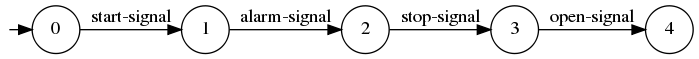
\includegraphics{src/2-framework/images/local-trace}}
\caption{LTS capturing the traces of the MSC of Fig.~\ref{image:train-scenario-all-agents} from the local point of view of the \artifact{Controller}.\label{image:local-traces-lts}}
\end{figure}

At first glance, a similar reasoning can be applied to the composed system. Indeed, one could consider that a MSC defines a \emph{maximal} trace in the composed system, with all events in a top-down ordering. In the example at hand, such a trace would be \artifact{<start-signal, start, alarm-pressed, \ldots, open>}. Making so amounts to consider that a MSC defines a total order among all events while it is commonly admitted that it defines only a partial order~\cite{ITU:1996, Uchitel:2003}. Consider for example the events \artifact{start-signal} and \artifact{alarm-pressed} at begining of the MSC. These two events model unrelated phenomena between different agents, and can therefore hardly be considered timely ordered (e.g. maybe does the passenger push the alarm button when the \artifact{start-signal} is already sent but before \artifact{start} has been propagated? or even before \artifact{start-signal}?, and so on.). 

Even when considering partial ordering of all events, it is possible to capture all MSC traces respecting the total orders defined by the agent timelines. These traces are called \emph{linearizations} of the MSC. We do not formalize the structure of Message Sequence Charts and their linearizations here, and refer the reader to~\cite{Uchitel:2003} for such a mathematical characterization. Semantically, we note however that the set of system traces of a single MSC $M$ with $n$ interacting agents -- also called its \emph{language} -- can be constructively captured by the following LTS composition:

\begin{equation}
\label{equation:msc-composition}
\mathcal{L}(M) = \mathcal{L}(M_{\downarrow Ag_1} \parallel \ldots \parallel M_{\downarrow Ag_n})
\end{equation}

\noindent where, for recall, $M_{\downarrow Ag_i}$ denotes a LTS like the one of Fig.~\ref{image:local-traces-lts} for the timeline of the $i$-th agent. From an implementation point of view, the previous LTS composition gives a simple way of computing all linearizations of a MSC as a transition system directly. Such a LTS is illustrated in Fig.~\ref{image:msc-linearizations} for the case at hand, where six different linearizations exist due to the possible interleavings of the first four events. The reader familiar with the related literature may wonder here if some of these traces should not be considered as \emph{implied} scenarios. Strictly speaking, that is according to the definition of an implied scenario given in~\cite{Uchitel:2004}, they are not. We discuss implied scenarios in section \ref{section:background-discussion}.

\vspace{0.5cm}
\begin{figure}[H]\centering
\scalebox{0.31}{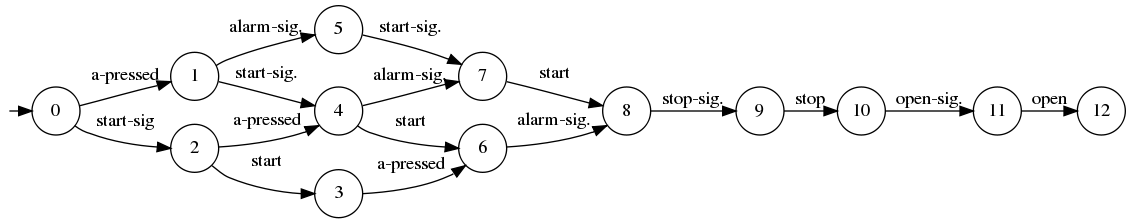
\includegraphics{src/2-framework/images/linearizations}}
\caption{LTS capturing all event linearizations of the MSC of Fig.~\ref{image:train-scenario-all-agents}. Here, \artifact{alarm-pressed} is abbreviated as \artifact{a-pressed} and \artifact{sig.} stands for \artifact{signal}. \label{image:msc-linearizations}}
\end{figure}

The semantics of a single MSC in terms of agent and system traces can now be explicitly related to the notion of the LTSs modeling the complete behavior of the agents and the system. That is, we can now explain the similitudes between definitions \ref{equation:system-composition} and \ref{equation:msc-composition} through the notion of MSC consistent with a system. 

Consider a system $S$ composed of $n$ agents whose behavior is modeled by the LTSs $Ag_1$ to $Ag_n$. Let $M$ denote a MSC illustrating interactions between them. We say that $M$ is \emph{consistent} with $S$ -- or, more accurately, that $M$ and $S$ \emph{are} consistent -- if the following conditions hold:

\begin{itemize}
\item $M$ and $S$ are \emph{architecturally} consistent,
\item $\mathcal{L}(M_{\downarrow Ag_i}) \subseteq \mathcal{L}(Ag_i)$ for each agent $Ag_i$, and
\item $\mathcal{L}(M_{\downarrow Ag_1} \parallel \ldots \parallel M_{\downarrow Ag_n}) \subseteq \mathcal{L}(Ag_1 \parallel \ldots \parallel Ag_n)$
\end{itemize}

The first condition is not formalized but simply requires the MSC and the system to agree on the set of agents (the MSC could actually be a proper subset) and their respective interfaces (labels along a timeline are a subset of the alphabet of the corresponding agent). The second condition states that the traces defined by a timeline in the MSC must be traces accepted in the LTS modeling the behavior of the corresponding agent. The third condition states that all linearizations of the MSC must be accepted traces of the LTS modeling the behavior of the composed system. Note that, under architectural consistency, the second condition implies the third one (see~\cite{Uchitel:2003} for details). Last, but not least, stated conditions restrict consistent MSCs to those starting in the system initial state.

\subsection{Negative scenarios}

Positive message sequence charts model \emph{positive} examples of behavior that the system is expected to exhibit. It is often convenient to be able to model the counterpart, that is examples of behavior that the system is expected -- even required -- \emph{not} to exhibit. Such proscribed behaviors are illustrated with negative MSCs~\cite{Uchitel:2004}. A negative MSC is simply a scenario whose last event is proscribed, as depicted by a crossed arrow below a dashed line. An example is given in Fig.~\ref{X}, that shows that the \artifact{Controller} may not open train doors immediately after having started it.

More precisely, a negative MSC is a pair $(M,e)$ where $M$ is a positive MSC and $e$ is a single event (given our simplifying assumption, the latter event can simply be denoted by its label $l = label(e)$). The positive scenario $M$ is called the $precondition$ and $e$ the \emph{proscribed event}. The intuitive semantics is that, once the precondition has occurred from the system initial state, $e$ may not be the (very) \emph{next} event in the system. We make this semantics fully precise now. A negative MSC $N = (M,e)$ defines a set of traces as follows:

\begin{equation*}
\mathcal{L}(N) = \{~w.l \mid w \in \mathcal{L}(M) \wedge l = label(e) \}
\end{equation*}

That is, traces of a negative MSC are traces of the precondition (given by definition~\ref{equation:msc-composition}) concatenated with the label of the proscribed event. Note that, such a definition implies that the precondition must occur completely for the proscribed event to be taken into account. In other words, partial orderings between the proscribed event and those in the precondition are not considered. This is the intended meaning of the dashed line separating them~\cite{Uchitel:2004}. 

Similarly to positive MSCs, we state conditions for a negative MSC $N = (M,e)$ and a system $S = (Ag_1 \parallel \ldots \parallel Ag_n)$ to be consistent, as follows:

\begin{itemize}
\item $N$ and $S$ are \emph{architecturally} consistent,
\item $M$ and $S$ are consistent, and
\item $\mathcal{L}(N) \not\subseteq \mathcal{L}(Ag_1 \parallel \ldots \parallel Ag_n)$
\end{itemize}

The first condition is similar to what has been said previously for positive MSCs. The second enforces the precondition to be a consistent (positive) MSC. The last one states that the system may not exhibit any trace captured by the negative MSC.

\subsection[Flowcharting scenarios in high-level MSCs]{Flowcharting scenarios in high-level Message Sequence Charts}

\section{Discussion\label{section:background-discussion}}
